% Importado desde: 2026-03-28_Dirac_2p1_desde_QW_Honeycomb.tex
\chapter{Derivacion Pedagogica: --- Hacia Dirac en \(2+1\) desde una quantum walk sobre geometria honeycomb/triangular}
\label{ch:dirac-2p1-desde-qw-honeycomb}

\section{Objetivo}

En el documento anterior dejamos listo el hilo conceptual:

\begin{enumerate}[leftmargin=*]
  \item quantum walk minima en \(1D\);
  \item split-step en \(1D\);
  \item paso natural a \(2D\);
  \item reorganizacion geometrica tipo honeycomb/triangular.
\end{enumerate}

Ahora queremos dar el siguiente paso de verdad: escribir una derivacion pedagogica de como aparece un Hamiltoniano efectivo de Dirac en \(2+1\) cuando la caminata ya respeta las tres direcciones naturales de la geometria de grafeno.

La idea no sera reproducir toda la construccion formal mas tecnica de la literatura, sino aislar el mecanismo central y dejarlo claro, paso a paso.

\section{La idea fisica en una frase}

Si en \(1D\) una quantum walk construia Dirac combinando
\begin{equation}
\text{mezcla interna} + \text{corrimiento en una direccion},
\end{equation}
entonces en una geometria tipo honeycomb la version natural es
\begin{equation}
\text{mezcla interna} + \text{corrimientos en tres direcciones oblicuas}.
\end{equation}

El milagro geometrico es que esas tres direcciones no son redundantes: al combinarse correctamente, reconstruyen una dinamica efectiva isotropa en dos dimensiones.

\section{Las tres direcciones naturales}

Tomamos exactamente las mismas direcciones de primeros vecinos que en grafeno:
\begin{equation}
\vdelta_1 = a(0,-1),
\qquad
\vdelta_2 = a\left(\frac{\sqrt{3}}{2},\frac{1}{2}\right),
\qquad
\vdelta_3 = a\left(-\frac{\sqrt{3}}{2},\frac{1}{2}\right).
\label{c03:eq:deltas}
\end{equation}

Sus vectores unitarios asociados son
\begin{equation}
\hat{\vdelta}_i=\frac{\vdelta_i}{a}.
\end{equation}

La propiedad mas importante es
\begin{equation}
\hat{\vdelta}_1+\hat{\vdelta}_2+\hat{\vdelta}_3=0.
\label{c03:eq:sumzero}
\end{equation}

Eso nos dice dos cosas a la vez:

\begin{enumerate}[leftmargin=*]
  \item la geometria esta organizada por tres direcciones;
  \item pero solo hay dos grados de libertad espaciales independientes.
\end{enumerate}

\begin{figure}[ht]
\centering
\begin{tikzpicture}[scale=1.5,>=Latex]
  \coordinate (O) at (0,0);
  \coordinate (D1) at (0,-1);
  \coordinate (D2) at (0.866,0.5);
  \coordinate (D3) at (-0.866,0.5);

  \fill[black] (O) circle (1.8pt);
  \draw[->,very thick,red!70!black] (O) -- (D1) node[midway,right] {\small \(\vdelta_1\)};
  \draw[->,very thick,green!60!black] (O) -- (D2) node[midway,above right] {\small \(\vdelta_2\)};
  \draw[->,very thick,blue!70!black] (O) -- (D3) node[midway,above left] {\small \(\vdelta_3\)};

  \draw[dashed,gray] (D2) -- ($(D2)+(D3)$);
  \draw[dashed,gray] (D3) -- ($(D2)+(D3)$);
  \draw[dashed,gray] (D1) -- ($(D2)+(D3)$);

  \node[below] at (0,-1.25) {\small tres direcciones de primeros vecinos};
  \node[above] at (0,1.15) {\small \(\vdelta_1+\vdelta_2+\vdelta_3=0\)};
\end{tikzpicture}
\caption{Geometria minima inspirada en grafeno. Las tres direcciones oblicuas son el ingrediente espacial central de la caminata.}
\label{c03:fig:three-directions}
\end{figure}

\section{La estructura interna del caminante}

Como en las quantum walks de una dimension, introducimos un espacio interno de dos componentes. La diferencia es que ahora no queremos asociarlo solo a \enquote{derecha/izquierda}, sino a un objeto espinorial efectivo sobre el cual actuan las matrices de Pauli.

El truco natural es asociar a cada direccion \(\hat{\vdelta}_i\) una matriz interna
\begin{equation}
\tau_i = \hat{\delta}_i^x \sigma_x + \hat{\delta}_i^y \sigma_y.
\label{c03:eq:taui}
\end{equation}

Es decir:
\begin{equation}
\tau_1 = -\sigma_y,
\qquad
\tau_2 = \frac{\sqrt{3}}{2}\sigma_x + \frac{1}{2}\sigma_y,
\qquad
\tau_3 = -\frac{\sqrt{3}}{2}\sigma_x + \frac{1}{2}\sigma_y.
\label{c03:eq:taus}
\end{equation}

Esta eleccion es bellisima por una razon simple: la estructura interna \(\tau_i\) sigue exactamente la misma geometria angular que las direcciones espaciales.

\section{Derivadas direccionales}

Para cada direccion definimos la derivada direccional
\begin{equation}
D_i = \hat{\vdelta}_i\cdot \nabla.
\label{c03:eq:Di}
\end{equation}

De forma explicita:
\begin{equation}
D_1 = -\partial_y,
\qquad
D_2 = \frac{\sqrt{3}}{2}\partial_x + \frac{1}{2}\partial_y,
\qquad
D_3 = -\frac{\sqrt{3}}{2}\partial_x + \frac{1}{2}\partial_y.
\label{c03:eq:Di-explicit}
\end{equation}

El punto fino es que la caminata no se propagara con \(\partial_x\) y \(\partial_y\) por separado, sino a lo largo de estas tres direcciones oblicuas.

\section{El paso unitario de la caminata}

\subsection{Subpasos orientados}

La forma mas transparente de escribir un paso elemental es como producto de tres subpasos direccionales y una mezcla de masa:
\begin{equation}
U = S_3\,S_2\,S_1\,C_m.
\label{c03:eq:Ufull}
\end{equation}

Aqui:

\begin{enumerate}[leftmargin=*]
  \item \(S_i\) propaga localmente en la direccion \(\hat{\vdelta}_i\);
  \item \(C_m\) introduce la mezcla interna responsable del termino de masa.
\end{enumerate}

Tomamos
\begin{equation}
S_i = \ee^{-\,\ii \varepsilon v\, \tau_i p_i},
\qquad
p_i = \hat{\vdelta}_i\cdot \vp,
\qquad
\vp = -\ii \nabla,
\label{c03:eq:Si}
\end{equation}
y
\begin{equation}
C_m = \ee^{-\,\ii \varepsilon m \sigma_z}.
\label{c03:eq:Cm}
\end{equation}

El parametro \(\varepsilon\) representa el tamano de un paso temporal pequeno.

\begin{figure}[ht]
\centering
\begin{tikzpicture}[>=Latex,node distance=1.05cm]
  \node[draw,rounded corners,fill=green!8,minimum width=1.8cm,minimum height=0.82cm] (c) {\(C_m\)};
  \node[draw,rounded corners,fill=green!8,minimum width=1.8cm,minimum height=0.82cm,right=of c] (s1) {\(S_1\)};
  \node[draw,rounded corners,fill=green!8,minimum width=1.8cm,minimum height=0.82cm,right=of s1] (s2) {\(S_2\)};
  \node[draw,rounded corners,fill=green!8,minimum width=1.8cm,minimum height=0.82cm,right=of s2] (s3) {\(S_3\)};
  \draw[->,thick] (c) -- (s1);
  \draw[->,thick] (s1) -- (s2);
  \draw[->,thick] (s2) -- (s3);
  \node[below=0.5cm of s2] {\small el paso completo recorre las tres direcciones locales};
\end{tikzpicture}
\caption{Un paso de la caminata honeycomb. No se mueve en ejes cartesianos, sino siguiendo las tres direcciones propias de la red.}
\label{c03:fig:step-sequence}
\end{figure}

\subsection{Expansión a primer orden}

Como queremos el limite efectivo, expandimos para \(\varepsilon\ll 1\):
\begin{equation}
S_i \simeq I - \ii \varepsilon v\, \tau_i p_i,
\qquad
C_m \simeq I - \ii \varepsilon m \sigma_z.
\end{equation}

Entonces
\begin{equation}
U \simeq
\left(I-\ii \varepsilon v \tau_3 p_3\right)
\left(I-\ii \varepsilon v \tau_2 p_2\right)
\left(I-\ii \varepsilon v \tau_1 p_1\right)
\left(I-\ii \varepsilon m \sigma_z\right).
\end{equation}

Reteniendo solo primer orden en \(\varepsilon\):
\begin{equation}
U \simeq I - \ii \varepsilon
\left[
v\sum_{i=1}^3 \tau_i p_i + m \sigma_z
\right].
\label{c03:eq:Uexp}
\end{equation}

Por comparacion con
\begin{equation}
U \simeq I - \ii \varepsilon H_{\text{eff}},
\end{equation}
identificamos
\begin{equation}
H_{\text{eff}} =
v\sum_{i=1}^3 \tau_i p_i + m \sigma_z.
\label{c03:eq:Heffraw}
\end{equation}

\section{La cuenta central}

Aqui esta la parte mas importante de todo el documento. Sustituimos \(\tau_i\) y \(p_i\) en la suma
\begin{equation}
\sum_{i=1}^3 \tau_i p_i
=
\sum_{i=1}^3 (\hat{\vdelta}_i\cdot \vsigma)(\hat{\vdelta}_i\cdot \vp).
\label{c03:eq:keysum}
\end{equation}

Escribiendo componentes:
\begin{equation}
\sum_{i=1}^3 (\hat{\vdelta}_i\cdot \vsigma)(\hat{\vdelta}_i\cdot \vp)
=
\sum_{i=1}^3 \hat{\delta}_i^a \hat{\delta}_i^b \sigma_a p_b,
\end{equation}
donde \(a,b\in\{x,y\}\).

La geometria de los tres vectores unitarios cumple la identidad tensorial
\begin{equation}
\sum_{i=1}^3 \hat{\delta}_i^a \hat{\delta}_i^b
=
\frac{3}{2}\,\delta^{ab}.
\label{c03:eq:tensorid}
\end{equation}

Por lo tanto,
\begin{equation}
\sum_{i=1}^3 \tau_i p_i
=
\frac{3}{2}\left(\sigma_x p_x + \sigma_y p_y\right).
\label{c03:eq:magic}
\end{equation}

Esta ecuacion es el corazon del mecanismo.

Lo que parecia una suma de tres propagaciones oblicuas se reorganiza exactamente como un operador de Dirac bidimensional isotropo.

\begin{figure}[ht]
\centering
\begin{tikzpicture}[>=Latex,node distance=1.25cm]
  \node[draw,rounded corners,fill=orange!10,minimum width=3.2cm,minimum height=0.9cm,align=center] (a) {\((\hat{\vdelta}_1\cdot \vsigma)(\hat{\vdelta}_1\cdot \vp)\)};
  \node[draw,rounded corners,fill=orange!10,minimum width=3.2cm,minimum height=0.9cm,align=center,right=of a] (b) {\((\hat{\vdelta}_2\cdot \vsigma)(\hat{\vdelta}_2\cdot \vp)\)};
  \node[draw,rounded corners,fill=orange!10,minimum width=3.2cm,minimum height=0.9cm,align=center,right=of b] (c) {\((\hat{\vdelta}_3\cdot \vsigma)(\hat{\vdelta}_3\cdot \vp)\)};
  \node[draw,rounded corners,fill=blue!6,minimum width=4.7cm,minimum height=1.0cm,align=center,below=1.4cm of b] (d) {\(\dfrac{3}{2}(\sigma_x p_x + \sigma_y p_y)\)};
  \draw[->,thick] (a) -- (d);
  \draw[->,thick] (b) -- (d);
  \draw[->,thick] (c) -- (d);
\end{tikzpicture}
\caption{Recombinacion del operador efectivo. Las tres direcciones oblicuas producen el operador bidimensional de Dirac.}
\label{c03:fig:recombination}
\end{figure}

\section{Hamiltoniano efectivo final}

Sustituyendo \eqref{c03:eq:magic} en \eqref{c03:eq:Heffraw}, obtenemos
\begin{equation}
H_{\text{eff}}
=
\frac{3v}{2}\left(\sigma_x p_x + \sigma_y p_y\right)+m\sigma_z.
\label{c03:eq:Hefffinal}
\end{equation}

Si definimos
\begin{equation}
v_F = \frac{3v}{2},
\end{equation}
queda
\begin{equation}
H_{\text{eff}}
=
v_F\left(\sigma_x p_x + \sigma_y p_y\right)+m\sigma_z.
\label{c03:eq:Diracfinal}
\end{equation}

Y eso es precisamente la forma canonica del Hamiltoniano de Dirac en \(2+1\).

Pasando a espacio real, con \(p_x=-\ii\partial_x\) y \(p_y=-\ii\partial_y\), la ecuacion efectiva toma la forma
\begin{equation}
\ii \partial_t \psi(x,y,t)
=
\left[
-\ii v_F\left(\sigma_x \partial_x + \sigma_y \partial_y\right)
+ m \sigma_z
\right]\psi(x,y,t).
\label{c03:eq:dirac21real}
\end{equation}

\section{Que papel juega honeycomb y que papel juega triangular}

Aqui conviene ser muy claros.

\begin{enumerate}[leftmargin=*]
  \item La \textbf{geometria triangular} entra a traves de las tres direcciones \(\vdelta_i\).
  \item La \textbf{intuicion honeycomb} entra porque esas tres direcciones son precisamente las de primeros vecinos de grafeno.
  \item La estructura de \textbf{dos componentes internas} hace el trabajo del espinor efectivo.
\end{enumerate}

En otras palabras, la caminata no copia literalmente el modelo \emph{tight-binding} de grafeno. Lo que hace es capturar su organizacion geometrica esencial y usarla para reconstruir un operador de Dirac efectivo.

\section{Relacion con el grafeno del capitulo anterior}

En el documento de grafeno obtuvimos
\begin{equation}
H_{\text{graphene}} \simeq v_F(\sigma_x q_x + \sigma_y q_y)
\end{equation}
cerca de un punto de Dirac.

Aqui obtuvimos
\begin{equation}
H_{\text{eff}}
=
v_F(\sigma_x p_x + \sigma_y p_y)+m\sigma_z.
\end{equation}

La comparacion es inmediata:

\begin{enumerate}[leftmargin=*]
  \item el termino cinetico es el mismo;
  \item la geometria de tres direcciones es la misma semilla espacial;
  \item el termino \(m\sigma_z\) describe la posibilidad de abrir gap en la teoria efectiva.
\end{enumerate}

Asi, la quantum walk honeycomb/triangular no es un tema aparte. Es una relectura unitaria y discreta del mismo mecanismo que en grafeno produce fermiones de Dirac de baja energia.

\begin{figure}[ht]
\centering
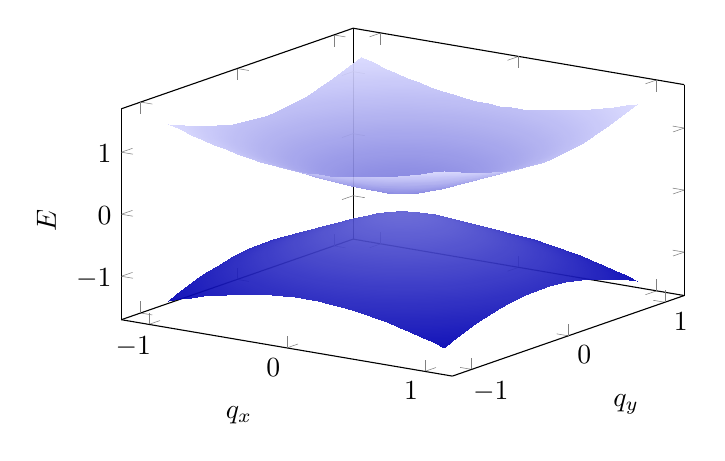
\begin{tikzpicture}
\begin{axis}[
  width=0.72\textwidth,
  height=6.0cm,
  xlabel={\(q_x\)},
  ylabel={\(q_y\)},
  zlabel={\(E\)},
  xmin=-1.2,xmax=1.2,
  ymin=-1.2,ymax=1.2,
  zmin=-1.7,zmax=1.7,
  samples=25,
  colormap={mycm}{color=(blue!70!black) color=(blue!15)},
  view={35}{25}
]
\addplot3[surf,shader=interp,opacity=0.92,domain=-1:1,y domain=-1:1]
  {sqrt(x^2+y^2+0.18^2)};
\addplot3[surf,shader=interp,opacity=0.92,domain=-1:1,y domain=-1:1]
  {-sqrt(x^2+y^2+0.18^2)};
\end{axis}
\end{tikzpicture}
\caption{Cono de Dirac con masa pequena. Cuando \(m=0\), el punto central es un nodo lineal exacto; cuando \(m\neq 0\), aparece un gap.}
\label{c03:fig:diraccone}
\end{figure}

\section{Lectura conceptual para el proyecto}

Este capitulo deja tres mensajes muy fuertes para la investigacion:

\begin{enumerate}[leftmargin=*]
  \item una caminata local y unitaria puede reconstruir un fermion de Dirac en \(2+1\);
  \item la geometria honeycomb no necesita imponerse como un detalle decorativo, sino que entra directamente en la estructura del operador efectivo;
  \item el paso desde grafeno hacia una discretizacion mas fundamental ya no parece un salto arbitrario: hay un puente matematico natural entre ambos lenguajes.
\end{enumerate}

Ese puente es exactamente lo que necesitabamos antes de pensar seriamente en el salto a \(3+1\).

\section{Mapa de continuidad}

\begin{figure}[ht]
\centering
\begin{tikzpicture}[>=Latex,node distance=1.3cm]
  \node[draw,rounded corners,fill=blue!6,minimum width=2.9cm,minimum height=0.92cm,align=center] (a) {QW minima\\\(1D\)};
  \node[draw,rounded corners,fill=blue!6,minimum width=2.9cm,minimum height=0.92cm,align=center,right=of a] (b) {split-step\\\(1D\)};
  \node[draw,rounded corners,fill=green!8,minimum width=3.1cm,minimum height=0.92cm,align=center,right=of b] (c) {QW honeycomb\\\(2D\)};
  \node[draw,rounded corners,fill=orange!10,minimum width=3.2cm,minimum height=0.92cm,align=center,right=of c] (d) {Dirac efectivo\\\(2+1\)};
  \node[draw,rounded corners,fill=purple!8,minimum width=3.3cm,minimum height=0.92cm,align=center,below=1.5cm of c] (e) {\(3+1\) discreto\\como paso siguiente};
  \draw[->,thick] (a) -- (b);
  \draw[->,thick] (b) -- (c);
  \draw[->,thick] (c) -- (d);
  \draw[->,thick] (d) -- (e);
\end{tikzpicture}
\caption{Ubicacion de este capitulo en el hilo general. La caminata honeycomb en \(2D\) funciona como el ultimo gran puente antes del bloque \(3+1\).}
\label{c03:fig:roadmap}
\end{figure}

\section{Resumen final}

La derivacion puede resumirse en cinco pasos:

\begin{enumerate}[leftmargin=*]
  \item tomar las tres direcciones \(\vdelta_i\) de la geometria de grafeno;
  \item asociar a cada una una matriz interna \(\tau_i=\hat{\vdelta}_i\cdot \vsigma\);
  \item construir el paso unitario como producto de tres propagaciones direccionales y un termino de masa;
  \item expandir el operador unitario a primer orden;
  \item usar la identidad geometrica \(\sum_i \hat{\delta}_i^a\hat{\delta}_i^b=\tfrac{3}{2}\delta^{ab}\) para recombinar todo como un operador de Dirac isotropo.
\end{enumerate}

Ese es el mecanismo esencial. Y justamente por ser tan claro, ya deja preparado el siguiente paso natural del proyecto: preguntar como imitar esta logica en \(3D\), donde en vez de tres direcciones coplanares habria que coordinar varias direcciones espaciales y una estructura espinorial mas rica.

